\chapter{Software Architecture Design\label{ch:Software Architecture Design}}
In this chapter, we will discuss the process of software architecture design. It is a crucial step of software engineering. A poor architecture might often result in low quality, reliability and maintainability. It also makes development more difficult. The architecture is hard to develop in an incremental way, and it is costly to change in the later stages. Therefore, enough attention should be paid to the architecture design.

\section{Layered Software Architecture}
There are different types of software architectures, such as layered architecture, event-driven architecture, micro-kernel architecture, micro-services architecture, cloud architecture etc. \cite{richards2015software}. The layered architecture is the most widely used, and the de facto standard software architecture.

The layered architecture contains roughly four layers: the presentation layer, the business layer, the persistence layer, and the database layer. The presentation layer is where the users interact with the software. It displays internal status of the software and receives user inputs. In case of a GUI software, the presentation layer consists of GUI widgets. The business layer is where a certain business logic is defined and implemented. The persistence layer, also known as data layer, is where the users access the database layer. The database connector API, for example, is on this layer. The bottom layer is the database layer containing SQL databases, files, and so on.

Each layer contains multiple modules that achieve a specific purpose. Within a specific layer, modules are fairly independent of each other. For example, we might want to define a dialog for adding new system blocks and another for adding registers. These two dialogs basically have nothing to do with each other. However, in practice, modules in a certain layer might also need to directly interact with non-neighboring layers. A well-designed layered architecture allows users to easily revise a certain module, or add a new module into a certain layer, without much modification on other modules on the same layer or neighboring layers.

\section{Layered Architecture Design}
With the layered architecture, what we need to do is divide the software into function modules and fill them into those layers. To design a good layered architecture, it is crucial to define good modules. We have to ask ourselves these questions:
\begin{itemize}
\item What modules should be there?
\item What is the boundary of each function module?
\end{itemize}

We found it might be a good idea to define modules by functionality. For each functionality, we create a UI module and a business logic module. We put them in the presentation layer and business layer respectively. The persistence layer and the database layer in our case is quite straightforward. Intuitively, user authentication shall be somewhere between the presentation layer and the business layer. When users do something on the GUI, the authenticator shall check whether the operation is legal, and determine whether to execute the corresponding business logic function or prompt an error message to the user. In fact, we also want the presentation layer to adjust its appearance according to the authentication. As a result, we decided we should modify the default four-layered architecture by adding an authentication layer between the presentation and the business layer.

Following what is discussed, we listed functionalities from the requirements. For many of those functionalities a certain UI component is required. Some functionalities might share a single UI component. For example, when we add or edit a system block, we need the same dialog. Finally, we designed the software architecture as in Figure \ref{fig:Layered Architecture}. Only part of the modules are included in the figure.

\begin{figure}[htb]
\centering
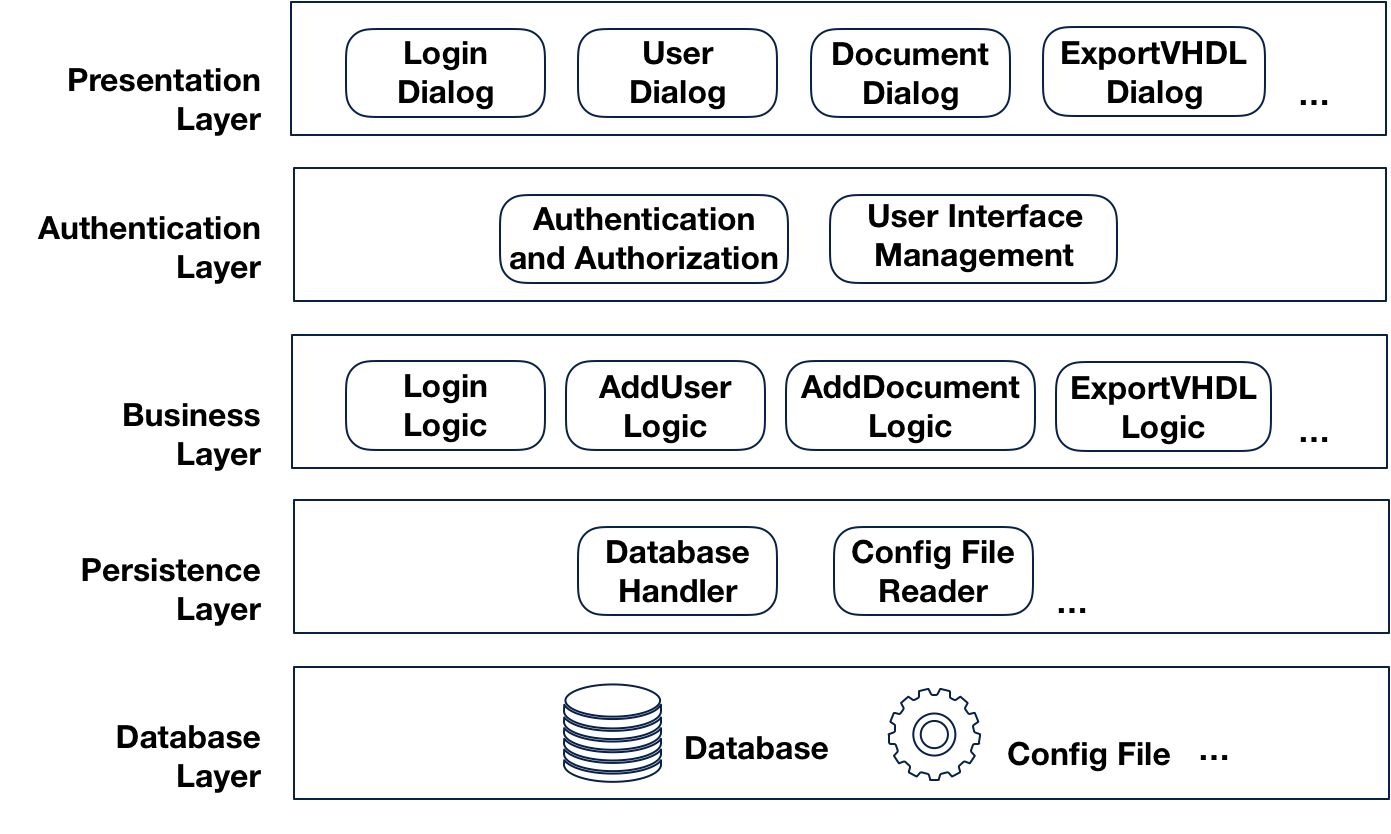
\includegraphics[width = \textwidth]{LayeredArchitecture}
\caption{Layered Architecture\label{fig:Layered Architecture}}
\end{figure}

\section{Object-Oriented System Design}
So far we designed the layered architecture of the software by dividing it into function modules, and assigning each module to a certain layer. The layered architecture, however, does not model the interactions between modules within a layer or across layers. Also, the models are not associated with any implementation form. In practice, they can be implemented with a class or a function. In this section, we will design the software system in more details following the object-oriented programming paradigm, and finally produce a class diagram. However, at this point we do not consider module design and implementation details. We will leave this to Chapter \ref{ch:Module Design and Implementation}.

\subsection{Object-Oriented Programming}
Object-oriented programming (OOP) is a programming paradigm based on objects. An object contains data and methods. Objects interact with each other and this usually leads to modification of the data in the objects. In the class-based OOP languages, an object is an instance of a class, a template for creating objects and providing initial values and behaviors. 

OOP has three central ideas \cite{eckel2003java}
\begin{itemize}
\item Encapsulation: the classes hide their internal status, and only expose necessary information.
\item Inheritance: it represents the \textit{is-a-type-of} relationship between classes.
\item Polymorphism: it provides a single interface to entities of different types.
\end{itemize}

The definition of classes and their relationships can be represented by the UML class diagram. The class is represented with a rectangle with three boxes as in Figure \ref{fig:Example Class}.
\begin{figure}[htb]
\centering
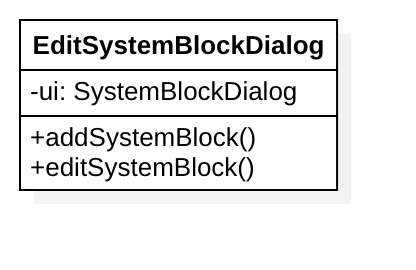
\includegraphics[width = 0.3\textwidth]{ExampleClass}
\caption{Example Class\label{fig:Example Class}}
\end{figure}
The top box contains the class name. The members variables (i.e. the data) are in the middle box. In the bottom box are member methods. The member variables and methods are decorated with +, \# or - representing public, protected and private respectively. Classes related to others are connected with lines of different forms as in Figure \ref{fig:Class Relationships}. Relationships can be categorized into instance-level and class-level. According to the degree of dependency, instance-level relationships are \textit{dependency}, \textit{association}, \textit{aggregation} and \textit{composition}. Dependency relationship exists when an instance references another. Association represents a \textit{has-a} relationship. Aggregation and composition are variants of the \textit{has-a} association relationship in that they represent a \textit{is-part-of} relationship. The difference is, the composition relationship entails ownership. If class A has a composition relationship with B, when B is destroyed A will be destroyed too. The class-level relationships reflect the inheritance relationships between classes. The two relationships differ in that realization involves an abstract superclass, aka an interface. 

\begin{figure}[htb]
\centering
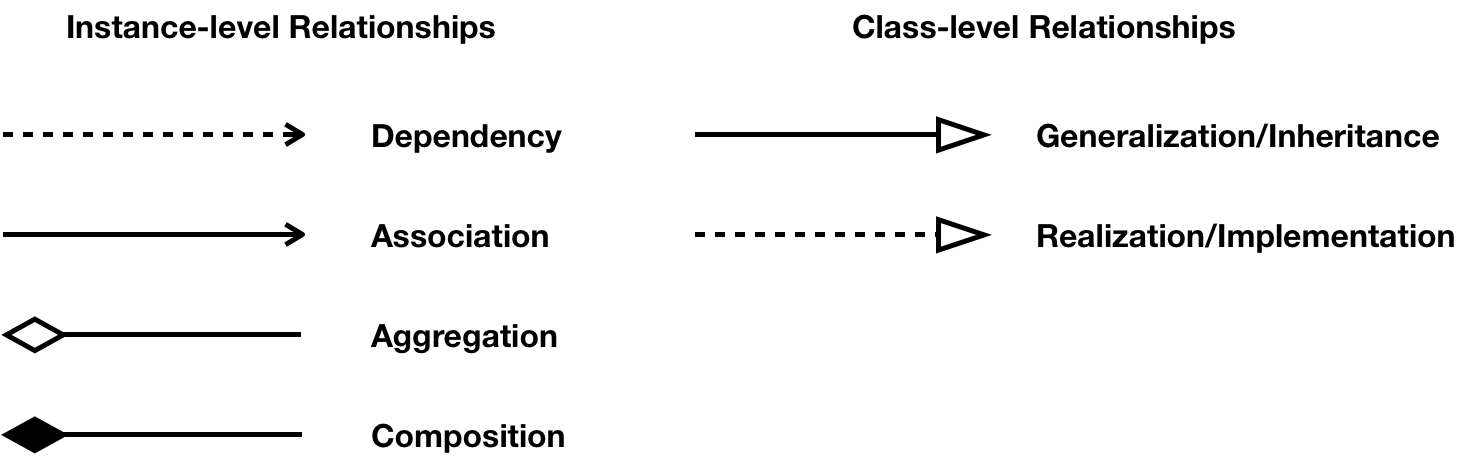
\includegraphics[width = 0.8\textwidth]{ClassRelationships}
\caption{Class Relationships\label{fig:Class Relationships}}
\end{figure}

\subsection{System Design}
With the OOP background, our task is to design the system and produce a class diagram.  At this point, we have to answer two questions
\begin{itemize}
\item What classes should there be and what are their functionalities?
\item What are their relationships with each other?
\end{itemize}
These two questions are not independent. The answer to one can influence the other.

In Qt, a general design pattern is to first design a UI form using the Qt Creator, and then design the class incorporating the UI as one of its member variable. We can design the UI in a WYSIWYG manner. The Qt Creator will then generate a UI form in XML format containing all information about the UI and a C++ class from the UI form. Then, we will create a class with an instance of the UI class. We can then write business logic functions in this class. In this way, modules in the presentation layer and business logic layers are unified. 

Some functionalities require user inputs. For example, to add a system block the name, abbreviation and start address of the system block must be given by the user. The client requires developers to design an appropriate dialog for such use cases. However, the dialog can be reused for different functionalities. The system dialog can be used for not only adding but also editing system blocks, for example. In such cases, a single UI class can be associated with multiple functionalities. Following the same pattern, we can design dialog classes for other functionalities such as adding or editing a signal, register and so on. Since these functionalities are independent of each other, these classes basically do not have relationships with each other, and we can design and implement them in an incremental manner.

According to the requirements, the main window shall contain a chip navigator, a chip editor view and a document editor view. Intuitively, we can design a \textbf{ChipNavigator}, \textbf{ChipEditorView} and \textbf{DocumentEditorView} class respectively. The \textbf{ChipEditorView} displays information about the chip and provides access to those functional dialogs related to chip editing. Similarly, the \textbf{DocumentEditorView} displays document items and provides access to document editing dialogs. The \textbf{MainWindow} itself is also associated with global level functional dialogs such as \textbf{SPIGenerationDialog}, \textbf{DocumentationGenerationDialog}, \textbf{ChangePasswordDialog} and so on. In the end, the system can be illustrated with the class diagram as shown in Figre \ref{fig:Register Manager Class Diagram}.

\begin{figure}[htb]
\centering
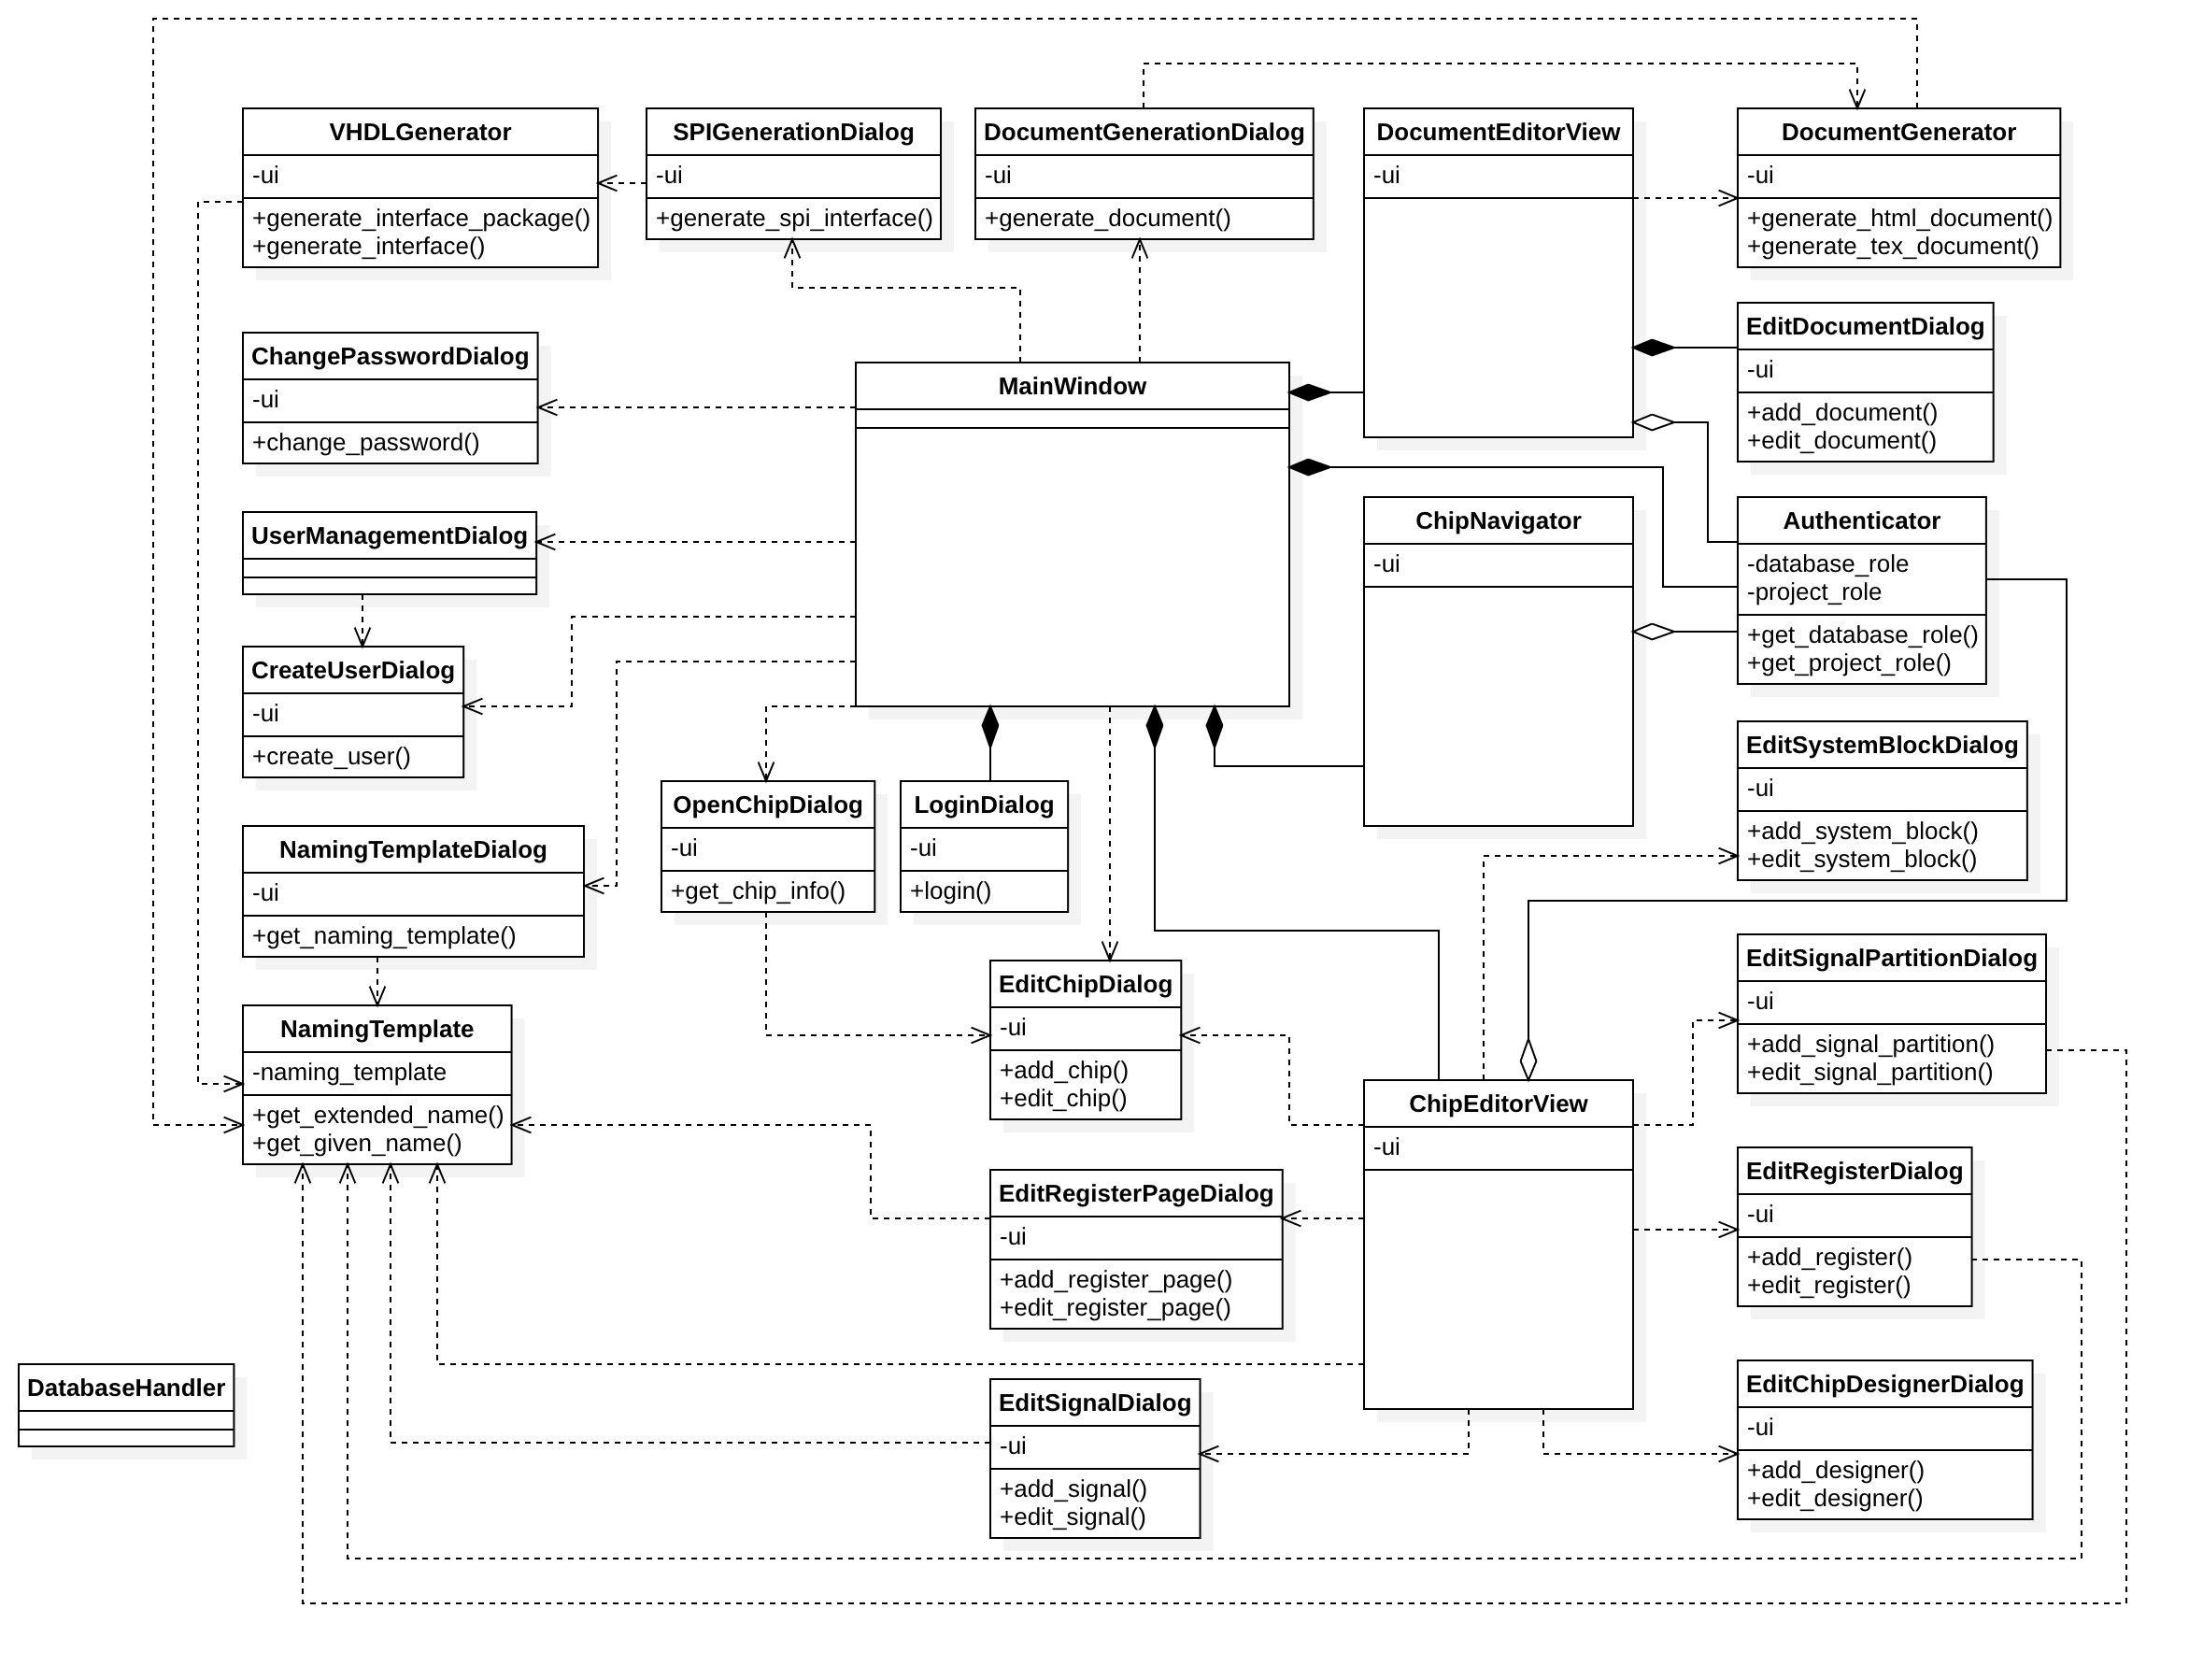
\includegraphics[width = \textwidth]{RegisterManagerClassDiagram}
\caption{Register Manager Class Diagram\label{fig:Register Manager Class Diagram}}
\end{figure}

Note that this class diagram is simplified in many ways. First, it only shows classes we want to create. The classes provided by Qt are omitted. The UI classes are not in the diagram either. Instead, they appear as a member named \textit{ui} of many classes in the diagram. Since we were still in the design phase so the classes were incomplete. Only the most important member variables and methods are shown in the diagram. Also, most classes have a dependency relationship with the \textbf{DatabaseHandler} class. However, their relationships are omitted in the diagram so as to make the diagram more readable and understandable.

The center of the software is the \textbf{MainWindow}. From the diagram we see that the \textbf{MainWindow} \textit{has} a \textbf{ChipNavigator}, \textbf{ChipEditorView}, \textbf{DocumentEditor}, \textbf{Authenticator} and a \textbf{LoginDialog}. Unlike other dialog classes such as \textbf{CreateUserDialog}, the \textbf{LoginDialog} is a member of the class \textbf{MainWindow} and it exits in the whole lifetime of the software (which is exactly the lifetime of the \textbf{MainWindow}). This is because we consider that users may want to log out and log in with another account. The \textbf{MainWindow} is directly dependent of many dialogs which are not directly associated to the \textbf{DocumentEditorView} or the \textbf{ChipEditorView}. These dialogs are not members of the class \textbf{MainWindow}. When they are needed, a certain action is triggered by the user and a temporary instance will be created.

The \textbf{ChipNavigator}, \textbf{ChipEditorView} and \textbf{DocumentEditorView} are members of the \textbf{MainWindow} and they exist in the whole life cycle of the software. The \textbf{ChipEditorView} are dependent of those chip editor dialogs including \textbf{EditChipDialog}, \textbf{EditSystemBlockDialog}, \textbf{EditRegisterDialog}. The \textbf{DocumentEditorView} is dependent of the \textbf{DocumentGenerator}. Likewise, these dialogs are created only when needed.

A special case is the \textbf{Authenticator}. It is the major component of the authentication layer. It stores the database permissions and project permissions of the current user to the current project. Whenever the current status changes, for example, when the user clicks on another system block on the navigator, permissions are requested and the UI is updated by enabling or disabling certain widgets. The \textbf{MainWindow} \textit{has} a member \textbf{Authenticator}. The pointer to the member \textbf{Authenticator} is passed to the \textbf{ChipNavigator}, \textbf{ChipEditorView} and \textbf{DocumentEditorView}, such that they actually access the same \textbf{Authenticator} instance.

Dependency relationships between the \textbf{MainWindow}, \textbf{ChipEditorView} etc. and the functional dialogs are easy and clear because those functional dialogs are basically independent of each other. However, the relationships between the \textbf{ChipNavigator} and the \textbf{ChipEditorView} or \textbf{DocumentEditorView} are tricky. In our design, they are not directly related to each other, but via the \textbf{MainWindow}. Whenever the user clicks on something in the navigator, it will \textit{tell} the \textbf{MainWindow} that something is triggered by sending it a \textbf{signal} (will be discussed in the Chapter \ref{ch:Introduction to Qt and SQL Programming}). The \textbf{MainWindow} then updates the current system block, register, signal etc., and updates the status of the \textbf{ChipEditorView} and \textbf{DocumentEditorView} by function calls. Likewise, when the chip is edited, the \textbf{ChipEditorView} sends a signal to the \textbf{MainWindow}. The \textbf{MainWindow} then calls a corresponding function to update the navigator.

To generate the SPI interface and the documentation, we use the \textbf{SPIGenerationDialog} and the \textbf{DocumentGenerationDialog}. With these dialogs, we can specify necessary inputs and configure the export. The \textbf{DocumentGenerationDialog} then creates a \textbf{DocumentGenerator} and calls the corresponding methods to create documentation rather in LaTeX or HTML (see Section \ref{sec:Document Generation}) format. Likewise, to generate the SPI interface, the \textbf{SPIGenerationDialog} creates a certain type of generator given the format of the export.

The \textbf{NamingTemplate} is designed in response to the requirement that the names of registers and signals shall be formatted. For example, we may want all register names to start with the block abbreviation and end with REG. To display the current naming templates, we use the \textbf{NamingTemplateDialog}, which also provides entries to editing the naming templates using the \textbf{EditNamingTemplateDialog}.

Although the class diagram does not regard how each class is implemented but only what functionalities they provide, we cannot design a software system completely without considering the design and implementation details of each class. We will discuss this in the Chapter \ref{ch:Module Design and Implementation}.